
Soient $n$ et $m$ deux entiers tels que $n < k$ et $m < k'$.
Consid\'erons une cellule $G_{n,m}$ qui contient $4$ sommets et $4$ ar\^etes.
Les sommets de  $G_{n,m}$  sont not\'es par les couples $(n,m)$, $(n,m+1)$, $(n+1,m)$,  $(n+1,m+1)$. 

% -----
Nous d\'esignons par 
\begin{itemize}
\item $e_{n} = \{(n,m),(n,m+1)\}$ l'ar\^ete entre les sommets $(n,m)$ et $(n,m+1)$,   
\item $e_{m} = \{(n,m),(n+1,m)\}$ l'ar\^ete entre les sommets $(n,m)$ et $(n+1,m)$,   
\item $e_{n+1} = \{(n+1,m),(n+1,m+1)\}$ l'ar\^ete entre les sommets $(n+1,m)$ et $(n+1,m+1)$,   
\item $e_{m+1} = \{(n,m+1),(n+1,m+1)\}$ l'ar\^ete entre les sommets $(n,m+1)$ et $(n+1,m+1)$.
\end{itemize}
Nous faisons varier $n$ et $m$ par pas de $1$ et nous s\'electionnons les cellules $G_{n,m}$ et $G_{n,m+1}$.
L'ar\^ete $e_{m+1}$ est commune aux cellules $G_{n,m}$ et $G_{n,m+1}$. 
De m\^eme, les cellules $G_{n,m}$ et $G_{n+1,m}$ partagent l'ar\^ete $e_{n+1}$. 
Ainsi, \`a chaque \'etape de la construction, chaque cellule partage 
$2$ ar\^etes si $n = m = 0$ ou $n = k-1 ~et~ m = k'-1$,
$3$ ar\^etes si $n = \{0,k-1\} ~et~ m \neq \{0,k'-1\}$ ou $m = \{0,k'-1\} ~et~ n \neq \{0,k-1\}$, 
$4$ ar\^etes si $n \neq \{0,k-1\} ~et~ m \neq \{0,k'-1\}$. 
\newline
\`A la fin de la boucle, nous ajoutons les ar\^etes $\{(0,0),(k+1,0)\}$, $\{(0,0),(0,k+1)\}$, $\{(k+1,k'+1),(k+1,0)\}$ et $\{(k+1,k'+1),(0,k+1)\}$.
Nous obtenons ainsi le graphe $G_{k,k'}$.
% -----

\begin{definition}
Le graphe $G_{k,k'}$ poss\`ede $(k+1) \times (k'+1)$ sommets,  $k \times (k'+1) + k' \times(k+1) + 4$  ar\^etes et $k \times k' +1$ cellules.
\end{definition}

% ---- figure exemple graphe cellule G_{3,3}
\begin{figure}[htb!] 
\centering
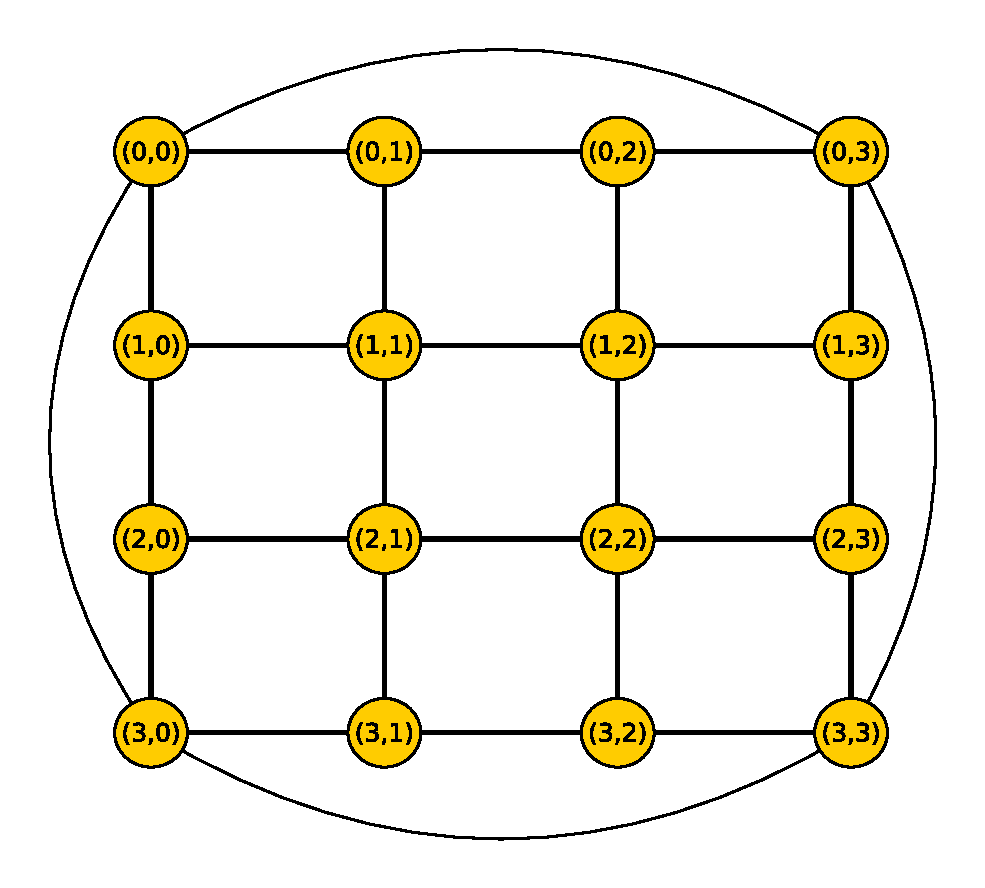
\includegraphics[scale=0.6]{exempleGrapheCelluleG33.eps}
\caption{ Le graphe cellule $G_{3,3}$ : il est compos\'e de $16$ sommets, $28$ ar\^etes et $9$ cellules. }
\label{exempleGrapheCellule} 
\end{figure}
%\FloatBarrier
% ---- figure exemple graphe cellule G_{3,3}

Dans la figure \ref{exempleGrapheCellule}, nous avons un exemple de graphe cellule $G_{3,3}$ avec $k=3$ et $k'=3$. Nous avons $16$ sommets, $28$ ar\^etes et $9$ cellules. 